\section{Results \& Discussion}
The software part of the line-following-robot started with high expectations of a working PID controller. However, our sensor boards had issues so only 2 sensor boards worked during the programming phase. This made PID control overly complex for our robot, so a reactive controller was made using Arduino programming, code in Appendix A. A limitation to having feedback from 2 sensors was the oscillations of the robot due to the sensors continuously triggering changes in direction without settling. This reduced the potential top speed of the robot. 
\\

To combat this, a third sensor positioned at the centre was added, and the robot moving forward when the sensor detected the line. By adding a third sensor, there was an average 4.9-second increase in course performance times, outlined in the ‘Course Times by Sensor Configurations and Weight’ table in Appendix B. This time saving was expected due to increased feedback allowing the sensors to occasionally settle in a forward state when the centre sensor detects the line. In doing so, the robot followed the line more smoothly, allowing for increased speeds. Therefore, to further reduce the average course time from a software perspective, a working PID and more sensors closely spaced together would be recommended. Weight was added to above the motors to increase the friction between the motors and wheels. Rough blotches of solder were also melted onto the motor shafts, which allowed it to grip the wheels better. Figure \ref{fig:Trialchart} shows the results of these optimisation changes. 

\begin{figure}[H]
    \centering
    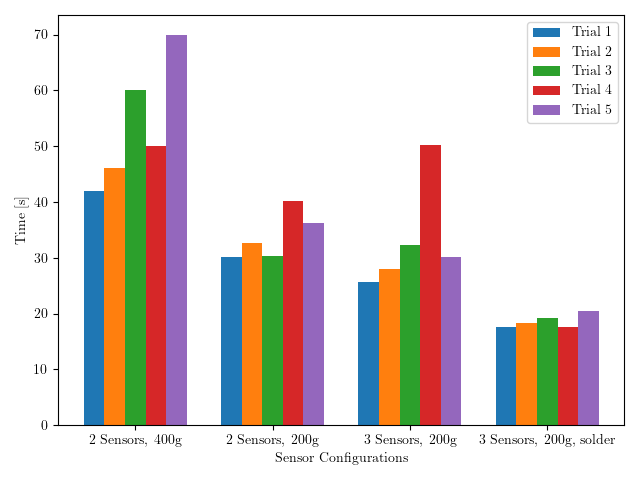
\includegraphics[width=0.5\linewidth]{REPORT/plotv3.png}
    \caption{Line Following Robot Course Times by Sensor Configurations and Weight }
    \label{fig:Trialchart}
\end{figure}

The Line Following Robot performed competitively well in the final demonstration, finishing the course in 14.939 seconds on our first attempt. A video of the robot's final run can be accessed with the following link: \href{https://youtu.be/P_ezBJ8gyDk}{$https://youtu.be/P_ezBJ8gyDk$}. The robot tracked the line reasonably accurately, with only minor overshooting when trying to make turns, which was within an acceptable range. After the first trial, we attempted to move the sensors closer together to improve line detection accuracy and reduce overshooting, thereby increasing speed. However, this approach failed during testing due to interference between the sensors when they were positioned too close to each other. 
\\

Our second solution was to gradually increase the forward speed of the robot. However, this caused other issues, such as difficulty in maintaining accurate line detection, which led to increased deviations from the path and potential loss of control. The robot struggled to respond quickly enough to changes in the line’s direction, resulting in more frequent overshooting of turns and ultimately decreasing its overall performance and reliability in navigating the course. We tried several speed settings but couldn’t achieve a result better than our first trial. Due to time pressure, we were unable to conduct another trial. 
\\

Looking ahead, several solutions could yield better results. First, we could program an additional sensor, allowing the robot to utilize four sensors for improved line tracking and reduced overshooting. Secondly, we were using bang-bang control, which only has two states, on or off based on whether the robot is on or off the line. Transitioning to a PID control system could enhance performance. Proportional control would respond to the current error (the difference between the desired position, centred on the line, and the current position), integral control would address the accumulation of past errors to eliminate steady-state error, and derivative control would predict future errors based on the rate of change, helping to dampen the system and reduce oscillations. This approach could allow our robot to increase speed while following the line more accurately and with less overshooting during turns. 
\\

Moving forward from this project, we have gained a better understanding of the importance of real-world testing. If this project were to be repeated, we would allocate more time toward improving the design of the PCB board and conducting thorough software testing. 